%%%
% Automatic Layout
%%%

\section{Automatisches Layout}
\label{sec:automatic-layout}

% Was bedeutet automatisches Layout?
% Algorithmen zum Layout von Diagrammen
% Algorithmus, das auf ein Diagramm angewendet wird und das die Layout-Eigenschaften berechnet
% Layout-Eigenschaften: Position, Größe der Knoten und Routing der Kanten [Arvo02]
% mit einem Knopfdruck im Nachhinein
% die Interaktion mit dem Diagramm fehlt
% kein direkter Einfluss auf das Ergebnis des Layout-Prozesses
% nicht geeignet für Änderungen im Diagramm -> muss nochmal gestartet werden
% (deutet darauf hin, dass) -> nicht intuitiv
% textbasiert: Anwendung auf textuelle Sprache vs. graphisch: Anwendung auf graphische Sprache
 
\subsection{Textbasierte Ansätze}

Unter den textbasierten Ansätzen für das automatische Layout sind Layout-Algorithmen zu verstehen, die als Eingabe eine Beschreibung des Diagramms in Textform erfordern und als Ausgabe eine graphische Repräsentation des Diagramms liefern. Intern wird in der Regel das eingelesene textuelle Modell in ein graphisches Modell transformiert, auf das die Layout-Funktion angewendet wird. Das Resultat besitzt einen statischen Charakter und somit vermisst dieser Ansatz jegliche Möglichkeit der Interaktion. Nachträglich ändern lässt sich das Diagramm nur durch Veränderung des Quelltexts und einen wiederholten Aufruf des Layout-Algorithmus.

\subsubsection{Graphzeichnen}

% TODO: Verweis auf "graph-basierte Diagramme"
Wie bereits im Abschnitt X beschrieben wurde, bilden Graphen eine Basis für viele Typen der Softwarediagrammen. Mit der graphischen Darstellung von Graphen beschäftigt sich die mathematische Disziplin des Graphzeichnens, deren Aufgabe es ist, Layout-Algorithmen zu entwerfen, die optimale Layouts in Hinsicht auf die ästhetischen Regeln zu erzeugen \cite{Maier12A-Pattern-based}. Diese Algorithmen werden in Tools und Bibliotheken implementiert, die entweder allein stehend genutzt (siehe unten) oder in andere Programme eingebaut (siehe Abschnitt \ref{subsec:automatic-layout-graphical-approaches}) werden können.

Ein bekanntes Beispiel der Tools für die Visualisierung von Graphen ist das ursprünglich von AT\&T entwickelte Softwarepaket Graphviz\footnote{\url{http://graphviz.org}}, das in diesem Abschnitt näher beschrieben wird. Es besteht aus folgenden Komponenten:

\begin{itemize}
    \item Domänenspezifische \textbf{Sprache Dot}\footnote{\url{http://www.graphviz.org/content/dot-language}} für die Beschreibung von Graphen.
    \item Ein Satz von \textbf{Layout-Algorithmen}.
    \item Ein Satz von \textbf{Kommandozeilen-Tools}\footnote{\url{http://www.graphviz.org/content/command-line-invocation}} für die Anwendung der Layout-Algorithmen und ihre grafische Ausgabe.
    \item Eine \textbf{Software-Bibliothek}, die die Funktionalität der Layout-Algorithmen und der graphischen Ausgabe bereitstellt und sich in andere Programme einbauen lässt \cite{Gansner14Using}.
\end{itemize}

Um einen Layout-Algorithmus auf einen Graph mit Hilfe der Komandozeilen-Tools anwenden zu können, muss der Graph in der Dot Sprache beschrieben werden. Ein Beispiel eines einfachen Graphen mit 4 Knoten und 3 Kanten ist im Quelltext \ref{lst:graphviz-dot-example-dot} gegeben.

\lstinputlisting[
    caption={Beschreibung eines Graphen in Dot (\lstinline{graphviz-dot-example.dot})},
    label={lst:graphviz-dot-example-dot}
]{resources/graphviz-dot-example.dot}

Mit dem Aufruf des Befehls aus dem Quelltext \ref{lst:grapviz-dot-example-sh} wird die oben aufgelistete Dot-Datei \lstinline{graphviz-dot-example.dot} eingelesen, der beschriebene Graph wird in ein internes Modell importiert, auf das der Layout-Algorithmus \lstinline{dot} angewendet wird. Anschließend wird mit dem Renderer \lstinline{png} ein Resultat in der PNG-Datei \lstinline{graphviz-dot-example.png} erzeugt, das in Abbildung \ref{fig:graphviz-dot-example} dargestellt ist \cite{Gansner14Using}.

\lstinputlisting[
    caption={Aufruf des Kommandozeilen-Tools \lstinline{dot}},
    label={lst:grapviz-dot-example-sh}
]{resources/graphviz-dot-example.sh}

\begin{figure}[hbt]
    \centering
    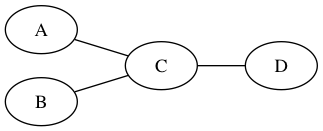
\includegraphics[scale=0.8]{resources/graphviz-dot-example.png}
    \caption{Resultat des Aufrufes des Kommandozeilen-Tools \lstinline{dot}}
    \label{fig:graphviz-dot-example}
\end{figure}


%% Layout-Eigenschaften (Parameter...)
%% etwas zu den Algorithmen
%% mathematische Algorithmen für Layout von Graphen


% TODO: Titel Generalisieren
\subsubsection{yUML}

% yUML.me, planttext.com, UMLGraph
% Text-Notation in Form einer DSL
% fehlende Interaktion des Nutzers mit dem Diagramm
% Veränderungen an einer anderen Stelle, keine unmittelbare Bearbeitung des Diagramms
% kein Einfluss auf das Layout

\subsection{Graphische Ansätze}
\label{subsec:automatic-layout-graphical-approaches}

Die graphischen Ansätze für das automatische Layout unterscheiden sich von den textbasierten darin, dass der Layout-Algorithmus auf eine graphische Sprache angewendet wird.

% unmittelbare Bearbeitung des Diagramms
% Ausführen des Diagramms im Nachhinein
% kein direkter Einfluss auf das Layout

% ---

% Graphviz

% Unterstützung des automatischen Layouts in OmniGraffle
% Interaktion mit dem Diagramm wird von dem Layout-Algorithmus nicht berücksichtigt => Zerstören des mentalen Modells
% Zusatzfunktion in OmniGraffle und CASE-Tools (Visual Paradigm anschauen)
% Graphviz Layout Engine

% Graphviz in Visual Paradigm

% ---

% Algorithmen für UML Klassendiagramme

% SugiBib - ein Framework, das auf dem Sugiyama Algorithmus basiert und die Semantik und Strukturregeln berücksichtigt
% https://wwwi2.informatik.uni-wuerzburg.de/SugiBib

% Kandinsky (Eiglsperger)

\subsection{Eigenschaften und Vergleich}

% Zusammenfassung
%% Verletzung der Semantik- und Strukturregeln durch die mathematischen Algorithmen
%% Interaktion im Vordergrund ist gewünscht
%% nicht geeignet für den Prozess des Zeichnens
%% Unterstützung der Diagrammtypen und deren Strukturregeln

%% Zerstören des mentalen Modells [Eiglsperger03 zitieren]
%% bei allgemeinen Algorithmen werden die Semantik- und Strukturregeln nicht berücksichtigt

%% Neuordnung des Layouts -> Zerstören der sekundären Notation [Seybold]

% Vorteile:
%% gute Ergebnisse für kleine und einfache Diagramme

% Nachteile:
%% fehlende Interaktion: Knopfdruck
%% Nutzer kann wenig beeinflussen
%% nicht für Änderungen geeignet -> Neustart
%% Semantik und Struktur...
%% berücksichtigen nicht die anwendugspezifische Einschränkungen [Gladisch]
%% Mangel an Möglichkeit der Kontrolle des Ergebnisses [Gladisch]
%% Nicht für interaktive Umgebung geeignet [Maier 2.4.1]


